\documentclass[11pt]{article}
\usepackage{ctex}

\usepackage[left=1.25in,right=1.25in,top=1in,bottom=1in]{geometry}
\usepackage{graphicx}
\graphicspath{{figures/}}
\usepackage{amsmath}
\usepackage{fontspec}
\usepackage{amssymb}

\begin{document}
	\title{数字图像处理(Didital Image Processing,DIP)}
	
	\maketitle
	
	\newpage
	\tableofcontents
	\newpage
	
\section{绪论}
\subsection{图像处理}

有些编码技术使得图片传输效率最大化,具有非常大的商业利益,可以保证大量复杂的硬件开发,例如:联合图像专家组(Joint Photographic Expert Group,JPEG),运动图像专家组(Moving Picture Expert Group,MPEG)等编码格式。C,C++,Java是目前为止最受欢迎的视觉系统实现语言,得益于它们在集成高级和低级功能方面力量强大而且编译能力强。随着系统变得越来越复杂,如果利用封装(encapsulation)和多型(polymorphism),C++和Java可以表现出更多的优越性。

\subsubsection{主要内容}

(1)数字图像处理

数字图像处理包括图像处理发展的历程,光和图像关系,人眼的视觉特性和图像质量评价方法

(2)图像数字化(Image Digitalization)

外部场景图像通过模拟图像的数字化处理,再使用计算机或其他数字设备进行处理。模拟图像数字化过程中最为关键的是取样,量化和编码这3个步骤。主要关注取样图像的混叠效应和图像的分辨率指标。

(3)图像变换(Image Transform)

利用正交变换改变图像数据结构,便于处理的特性,将图像转换到变换域中进行分析或处理。大多数的变换都有快速实现的方法,大大的提高了处理运算的速度。主要关注多种变换和分析的原理,特性,模型和快速实现的方法。

(4)图像增强(Image Enhancement)

按照人们的主观要对对目标图像进行处理,主要利用数学方法和各种变换手段。主要关注图像的灰度修正,图像平滑,噪声去除,边缘增强,特殊图像(如雾天图像,暗光图像)增强等。

(5)图像复原(Image Restoration)

把降质图像尽可能的恢复成原来的图像,是一类以客观指标为准的图像处理方法。主要关注对图像降质因素和降质模型的分析,以及针对降质模型的多种复原处理方法,包括无约束复原,有约束复原,非线性复原以及几何校正。

(6)小波变换(Wavelet Transform)

小波变换是一种局部化时频率分析方法,有许多优良特性:多尺度分解性,时频联合分析,方向选择,对象的自适应性。主要关注小波变换的原理和方法,多分辨率分析的基本内容和离散小波变换及其应用。

(7)图像压缩(Image Compression)

在满足一定图像质量要求的前提下,最大限度地压缩图像的数据量。以便存储更多的图像,或者图像传输节省更多的带宽。主要关注静止图像和活动图像的压缩方法(预测编码,变换编码和熵编码),以及指导图像压缩的信息熵概念和有限失真编码定理等。

(8)图像分割(Image Segmentation)

按照具体应用的要求将图像中有意义或感兴趣的部分分离或提取出来,这种分离或提取是根据图像的各种特征或属性进行的。图像分割经常是模式识别和图像分析的前处理阶段。主要关注经典的基于阈值,边界和区域的分割,以及较新的基于遗传算法的分割。

(9)图像描述(Image Description)和图像配准(Image Registration)

图像描述指用简单明确的数值,符号,图形或它们的组合表达图像的目标或区域的特征,以及区域之间的关系等。图像配准是通过比对同一场景不同图像的特征,将这些图像的几何位置上进行配准,以便综合利用多幅图像中的信息满足一定的应用场景。主要关注图像的边界描述,区域描述,基于特征的图像配准,SIFT配准和SURF配准。

(10)彩色图像处理(Color Image Processing)

在灰度图像处理的基础上,针对图像的彩色特性进行处理就形成了独特特点的彩色图像处理。主要关注不同彩色空间的基本构成和转换,彩色图像的平衡,增强,分割等基本处理方法。

(11)形态学图像处理(Color Image Processing)

用集合来描述图像目标及图像各部分之间的关系,说明目标的结构特点。在形态学图像处理中,设立结构元素来度量和提取图像中的对应形状,已到达对图像进行分析和识别的目的。主要关注二值图像和灰度图像的形态学处理两部分,腐蚀和膨胀两种基本形态学运算方法。

(12)基于偏微分方程的图像处理(Image Processing based on Partial Differential Equation)

针对图像空间域内像素点灰度值建立一阶,二阶或高阶微分方程,以此来表征图像中的区域纹理或边界等特征。通过PDE数值解方法可以在图像处理的同时较好地保持图像的原有特征。主要关注基于PDE的图像去噪,分割,放大和修复等处理方法。

(13)超分辨率重建(SRR,Super Resolution Reconstruction)

图像超分辨率技术(空间分辨率成倍增加)与图像恢复技术(分辨率不变)的目标都是重建高质量的原图像。主要关注基于插值,基于重建和基于学习的3类超分辨率图像重建方法。

(14)人工神经网络(ANN,Artificial Neural Network)图像处理

从信息处理的角度对人脑神经元进行抽象和模仿,建立某种简单模型,按不同的连接方式组成不同的信息处理网络。
主要关注基本结构和工作原理,基本的反向传播(BP, Back Propagation),卷积神经网络(CNN, Convolutional Neural Network)和生成对抗网络(GAN,Generative Adversarial Network)。

(15)图像的压缩感知(CS,Compressed Sensing)

基于信号稀疏性的压缩方法。将常规的取样,压缩两个步骤合并一起完成;对于压缩感知产生的压缩信号,通过适当的非线性重建算法可准确地重建原信号。主要关注信号的稀疏表示,非相关测量,感知信号非线性重建以及视频信号的分块压缩感知方法。
\subsection{图像数学表达}

图像其实是利用二维坐标指定的空间数据,计算机图像是一个像素矩阵(二维数组)。摄像机获取的是坐标x,y处像素点的亮度。通常,x和y分别表示水平轴和垂直轴。摄像机所获取的亮度被转换为信号,在经过A/D转换器处理,作为一个值存储在计算机内,可通过图像坐标x,y进行查询(reference)。计算机图像是一个点阵。灰度图像中每个点的值与摄像机所获得的场景中对应点的亮度值成正比。这些点就是图像元素,即像素。这些数据由储存在计算机里的数据点组成,数据为离散的。

像素矩阵,也就是图像,通常为方形的,一帧图像可以描述成$N\times N$的m位像素,其中N是点的数目,m表示亮度值的级数。
\subsection{图像质量评价}

图像质量含义:1.图像的逼真度,即被评价图像与原标准图像的偏离程度。2.图像的可懂度,是指图像向人或机器提供信息的能力。

在所有的评价方法中,按照是否需要参考图像分为:无参考(NR,No Reference)评价,部分参考(RR,Reduced Reference)评价和全参考(FR,Full Reference)评价

\subsubsection{主观评价指标}

人们对一幅图像视觉感受的主观评价,人自身对图像的评价是最为准确的。以国际电联ITU-R关于电视图像主观质量评价BT.500-13标准中的平均意见分(MOS,Mean Opinion Score)为基础的人眼观察评分的方法。

\begin{figure}[h]
	\centering
	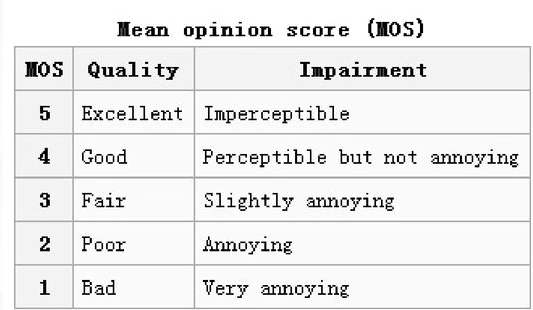
\includegraphics[scale = 0.5]{MOS}
\end{figure}

\subsubsection{客观评价指标}

客观评价方法:1.ITU-R视频质量专家组(VQEG,Video Quality Expert Group)规定的计算像素平均误差的客观质量评价方法。2.考虑人眼视觉特性的计算结构相似度的客观质量评价方法。

1.基于像素误差的评价

对于数字图像,设f(m,n)为原参考图像,$\hat{f}$(m,n)为其失真图像,尺度皆为MxN,定义失真图像的均方误差值(MSE,Mean Square Error)为
$$MSE = \frac{1}{MN}\sum_{n=1}^{N}\sum_{m=1}^{M}[f(m,n)-\hat{f}(m,n)]^2$$
在MSE的基础上定义失真图像的峰值信噪比(PSNR,Peak Signal Noise Ratio)为
$$PSNR = 10\cdot lg \frac{A^2}{MSE}(db)$$
其中A为原图像的最大灰度值。

所具有的局限性:1.需要原始图像进行对比。2.不一定能够准确地反映主观图像质量值,相同的PSNR值并不一定表示其主观质量一样,主观上好的图像不一定PSNR值高。

2.基于结构相似度的评价

基于结构相似度(SSIM,Structure Similarity)图像质量评价方法认为,相对于亮度和对比度信息,人类视觉系统对图像中的结构信息高度敏感,具有自动从视觉感知中提取结构信息的能力,因此结构信息量的变化能够反映一幅图像视觉感知失真的程度。而且,从图像形成的角度上来看,结构信息反映了场景中物体的结构,它基本独立于图像的亮度和对比度,亮度或对比度的改变对图像结构信息影响不大。

SSIM的比较对象为两幅灰度图像X和Y,其中一幅为参考图像,另一幅为其失真图像。设x为图像X的像素,y为图像Y的像素,两者的总像素为N,l(X,Y)为它们的亮度比较式,c(X,Y)是对比度比较式,s(X,Y)是结构比较式,定义如下:
$$l(X,Y)=\frac{2\mu_X\mu_Y+c_1}{\mu_X^2+\mu_Y^2+c_1}$$
$$c(X,Y)=\frac{2\sigma_X\sigma_Y+c_2}{\sigma_X^2+\sigma_Y^2+c_2}$$
$$s(X,Y)=\frac{\sigma_{XY}+c_3}{\sigma_X\sigma_Y+c_3}$$
将上述的各式组合起来成为图像X和Y的SSIM指数。
$$SSIM(X,Y)=[l(X,Y)]^{\alpha}[c(X,Y)]^{\beta}[s(X,Y)]^{\gamma}$$
为了简化表达,设定$\alpha =\beta = \gamma = 1$,且$c_3=\frac{c_2}{2}$,则SSIM指数为:
$$SSIM(X,Y)=\frac{(2\mu_X\mu_Y+c_1)(2\sigma_{XY}+c_2)}{(\mu_X^2+\mu_Y^2+c_1)(\sigma_X^2+\sigma_Y^2+c_2)}$$

由于图像统计特征通常是非全局平稳的,对整幅图像计算SSIM指数不如局部分块的效果好。例如,把图像分成不重叠的$8\times8$的小块,分块计算它们的SSIM值,整幅图像的SSIM值由各块的测量值加权平均得到,也可以简单平均得到。
$$SSIM(X,Y)=\frac{1}{M}\sum_{j=1}^{M}SSIM(bx_j,by_j)$$
其中X和Y分别是参考图像和失真图像,$bx_j$和$by_j$分别为X,Y对应位置的第j个小块,M是图像的小块个数。

目前相对成熟的是对黑白图像质量的定量评价,而对彩色图像在实用中往往将彩色图像的各个彩色分量作为灰度图像来评价,所有分量图像质量的平均就是该彩色图像的质量评分。

\subsection{其他评价方法}
\subsubsection{基于感兴趣区域的评价}
在进行PSNR计算时,对人眼感兴趣区域的像素给予更大的权值,加重ROI(Region of Interest)对图像质量结果的影响。这种方法较通常对整幅图像的所有像素平等对待更为合理(符合人眼的视觉心理要求)。
\subsubsection{联合视听评价}
一般情况下,我们在观看视频时都伴有声音,此时对图像质量的评价往往需要联合考虑音频和视频质量之间的相互作用。有以下结论:1.音频质量和视频质量共同贡献于整体的视听质量。2.一般情况下总体质量中视频质量占优势,而在音频和视频编码比特率都很低的情况下,或者视频质量已经大于某个门限值时,音频质量比视频质量更重要,并且随着音频质量的降低在总体质量中的影响逐渐增加。3.某些应用场景下,音频比视频内容更为重要。4.视听质量还会被其他因素影响,包括运动信息和视频内容的复杂性。
\subsubsection{无参考图像的评价}
在实际应用中,经常得不到参考图像或者获得参考图像的代价太大,因而要求评价方法降低对参考图像的依赖程度。经验表明,有时并不需要参考图像也能够对图像质量做出合理的评价,只要观测者在进行评价时抓住反映图像质量最本质的特征,如平滑程度,细节可分辨程度,彩色鲜艳程度。目前较为成熟的方法有面向特定失真和面向非特定失真的两类评价方法。特定失真有模糊失真,噪声干扰,块效应失真,JPEG压缩失真等。
\subsubsection{基于机器学习的评价}
机器学习作为一种数据驱动型的智能化信号处理工具已经开始应用于图像质量评价邻域,出现了多种接近主观评价的图像质量评价算法。如基于支持向量机(SVM,Support Vector Machine)分类器的训练,通过分析小波系数来提取图像中的特征。
\section{数字图像基础}
常见的图像处理是在以计算机为中心的,包括多种输入,输出,储存,传输及显示设备在内的数字图像处理系统上进行的。目前常用的图像分为两类:1.连续(或模拟)图像,如从传统照相机,摄像机获得的图像;2.直接获得数字图像,如数码相机,数字摄像机等。
\subsection{连续图像函数}
图像是通常意义下光辐射和场景物体反射的共同结果,用辐射的强度,即图像的亮度表示光强度的空间分布,形成空间坐标(x,y,z)的函数,如$f(x,y,z)$。

一幅彩色图像,各点值还应反应出色彩变化,用$f(x,y,z,\lambda)$表示,$\lambda$为波长。

一幅活动的彩色图像,还应是时间t的函数,可以表示为连续的多维函数。
$$I = f(x,y,z,\lambda,t)$$
其中,x,y,z表示空间某点的坐标,t为时间轴,$\lambda$为光的波长。

在现实世界中,由于I表示的是物体反射,投射或辐射的光能量,所以I为一个非负,连续的有限函数,即$0\le I\le I_{MAX}$。其中$I_MAX$表示I的最大亮度值,一般I=0表示黑色,负的亮度值一般 没有实际的物理意义。 

人眼所能够感知的景物一般必须是连续的,以此不管中间过程如何用数字的方法进行处理,最终提交给眼睛的图片必须是连续的,即连续图像或模拟图像。
\subsection{常见图像种类}
\begin{figure}[h]
	\centering
	\rotatebox[origin=c]{90}{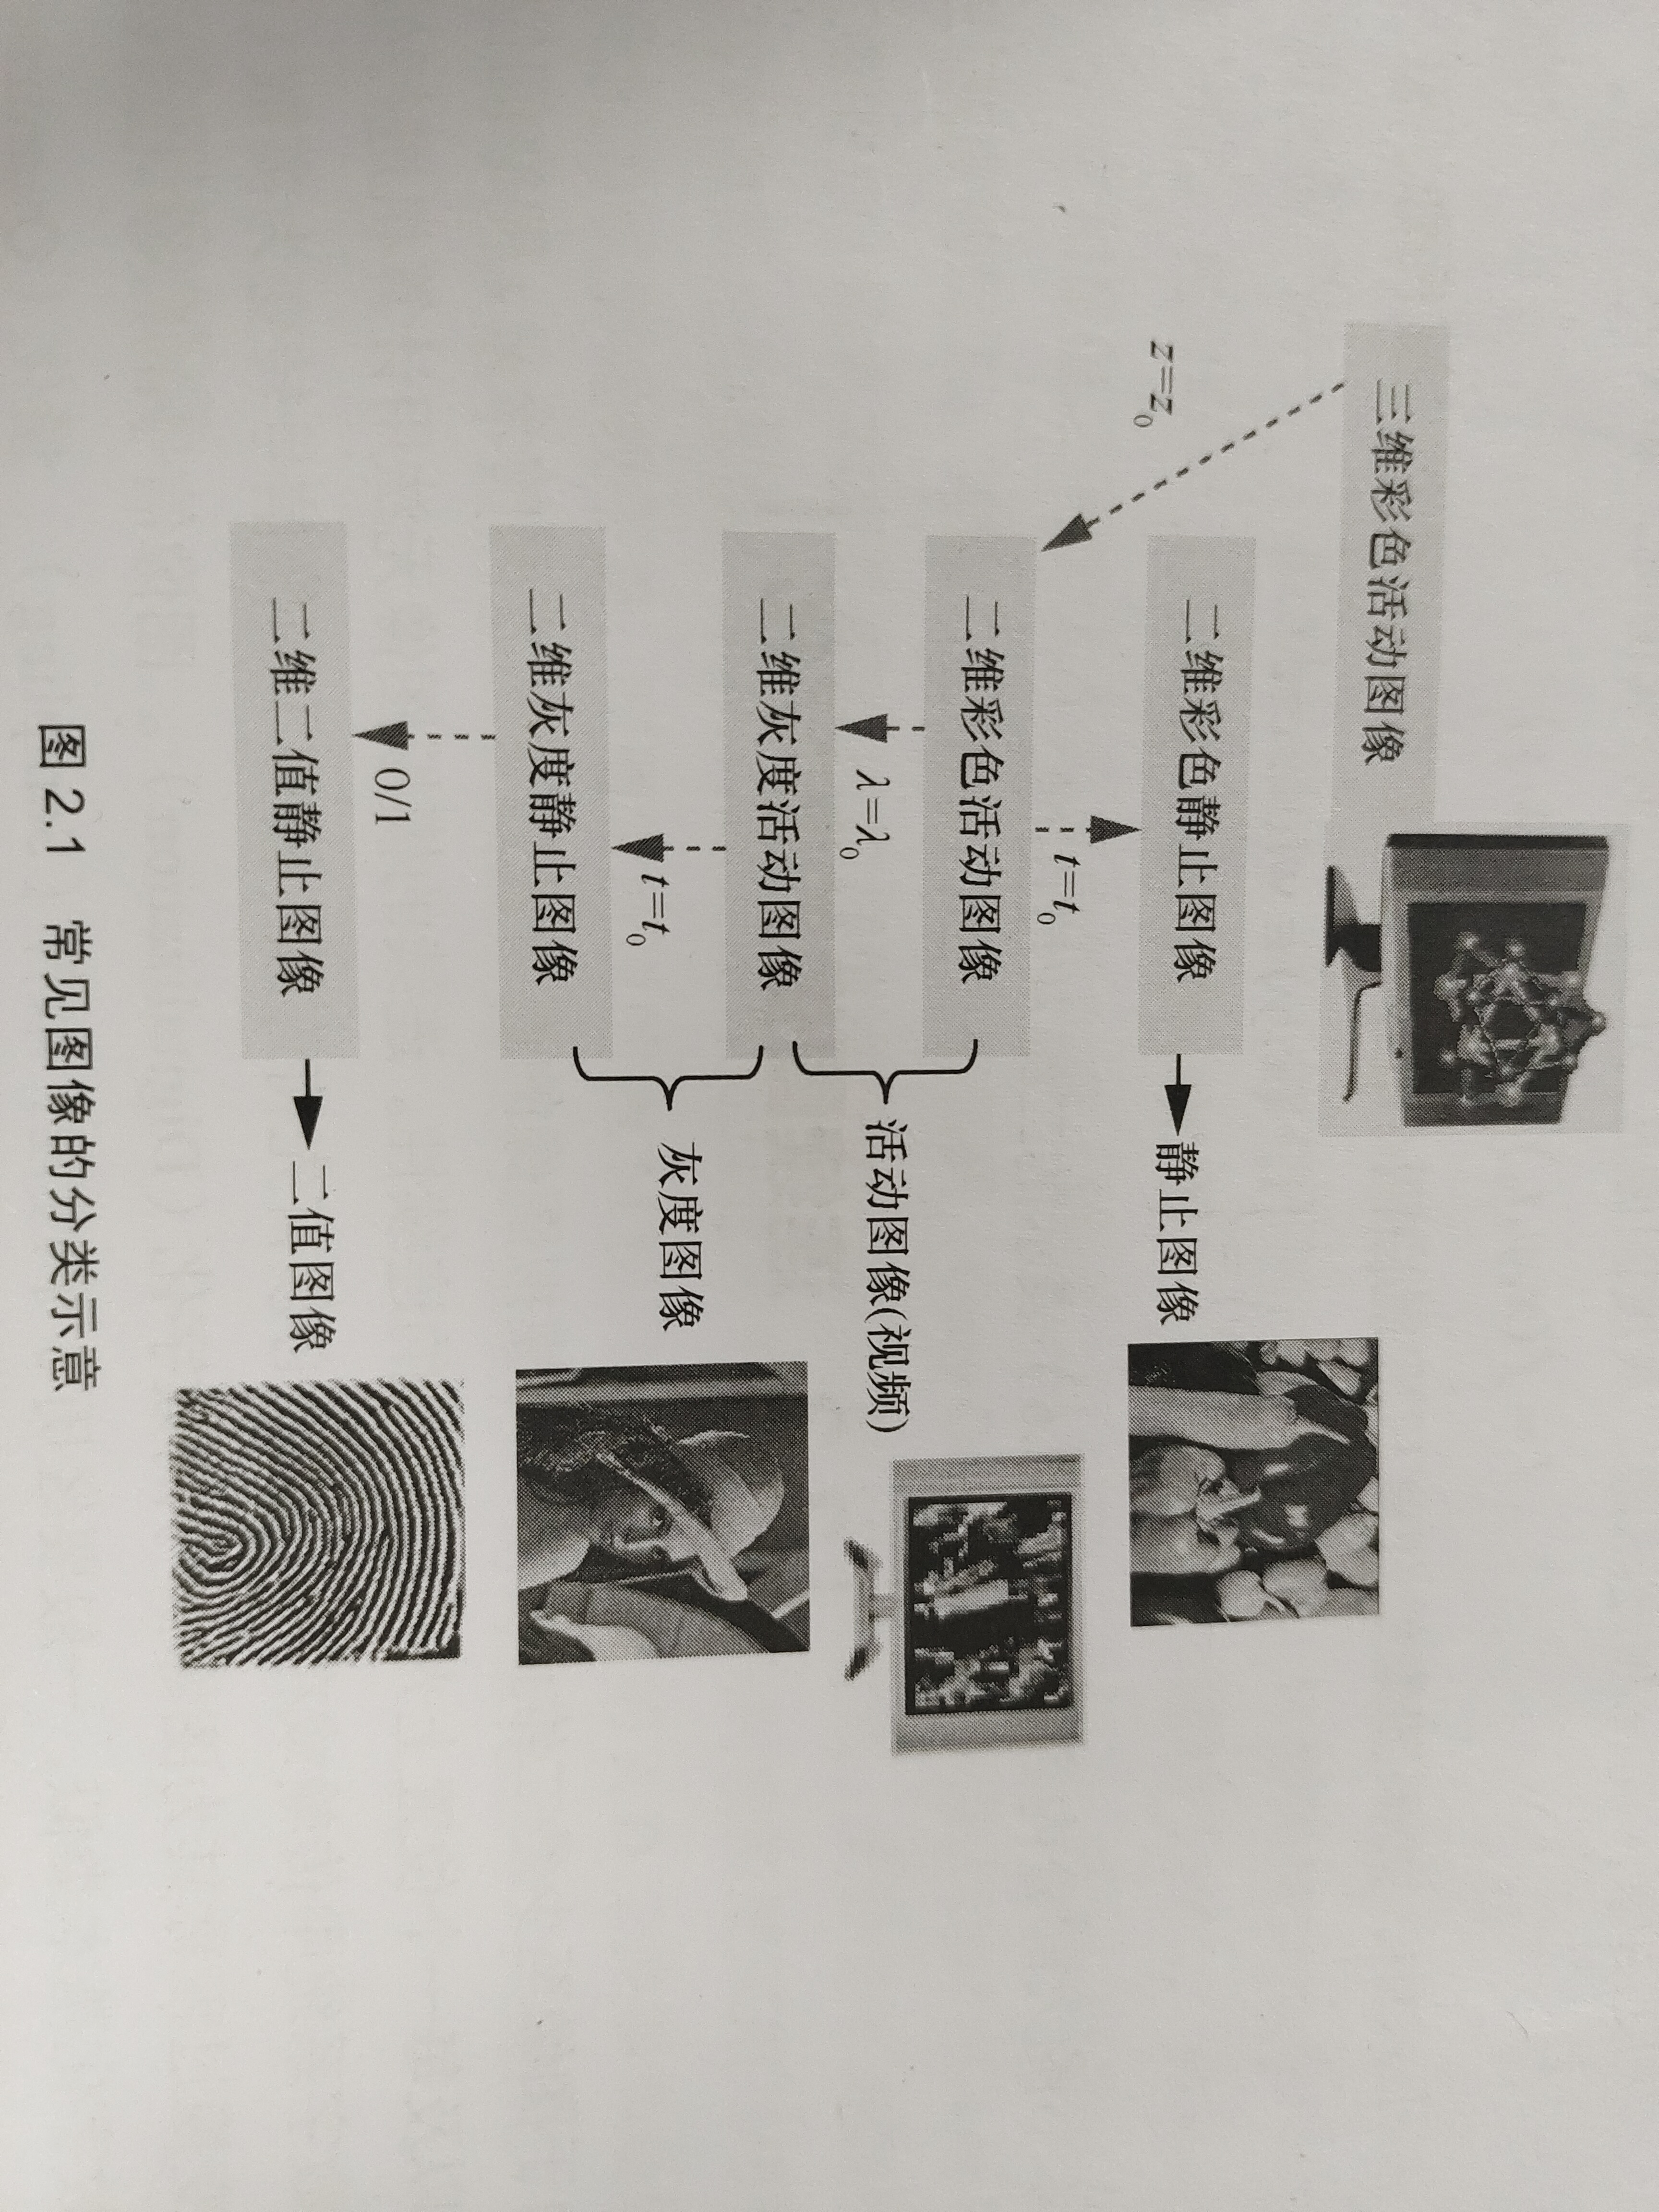
\includegraphics[scale=0.06]{1}}
\end{figure}
一个三维,彩色,活动的图像:
$$I = f(x,y,z,\lambda,t)$$

取$z=z_0$时,或不考虑深度信息时,则表示为一个二维,彩色,活动的图像:

$$I = f(x,y,z_0,\lambda,t)\qquad \text{或} \qquad I = f(x,y,\lambda,t)$$

取$t=t_0$时,图像内容不随时间变化,则表示为二维,静止的彩色图像:
$$I = f(x,y,\lambda,t_0) \qquad \text{或} \qquad I = f(x,y,\lambda)$$

可根据红黄蓝(RGB,Red Green Blue)三基色原理,将$I$分解为3个基色分量图像$I_R,I_G,I_B$:
$$
\left\{\begin{matrix}
	I_R = f_R(x,y,\lambda_R) \\ 
	I_G = f_G(x,y,\lambda_G) \\
	I_B = f_B(x,y,\lambda_B) \\
\end{matrix}\right.
$$
其中,$\lambda_R,\lambda_G,\lambda_B$为3个基色波长。

取$\lambda = \lambda_0$,当$\lambda$取为定值时,表示单色图像,则表示为二维,活动,灰度(单色)图像:
$$I = f(x,y,\lambda_0,t)\qquad \text{或} \qquad I = f(x,y,t)$$

取$t=t_0$,或者图像内容不随时间变化,则表示二维,静止,灰度图像,简称灰度图像:
$$I = f(x,y,t_0)\qquad \text{或} \qquad I = f(x,y)$$

在上式中,如果灰度只取黑白两个值,就形成了二值图像:
$$I = f(x,y) = \left\{\begin{matrix}
	1, \qquad (x,y)\in white\ erea \\ 
	0, \qquad (x,y)\in black\ erea \\
\end{matrix}\right.$$
\subsection{连续图像的数字化}
图像信号的数字化过程和其他模拟信号数字化过程基本相似,一般要经历3个过程:取样(Sampling),量化(Quantization)和编码(Coding)。

(1)取样(二维奈奎斯特取样定理)

图像$f(x,y)$的定义域在二维空间(x-y平面)上的离散化过程称为取样或抽样。被选取的点称为取样点,抽样点或样点,这些取样点也称为像素(pixel)。在取样点上的函数值称为取样值,抽样值或样值。取样就是在定义域空间(图像)上用有限的取样点来代替连续无限的坐标值。

(2)量化(操作完后一定失真)

对每个取样点函数值(灰度)的离散化过程为量化。即用有限个数值来代替连续无限多的灰度值。量化两大类,1.将每个样值独立进行量化的标准量化(Scaling Quantization),还可继续分为均匀量化(将样点灰度值等间隔分档,通常采用的是编码中的PCM编码),非均匀量化(不等间隔分档)。2.将若干样值联合起来作为一个矢量来量化的矢量量化(Vector Quantization)。

(3)编码

将经过量化后的离散灰度值用适当的二进制(或其他进制)数来表示。有不同的编码方法,只要保证量值和号码之间的对应关系即可。常见的编码方法有:PCA(Pulse Code Modulation)脉冲编码调制,格雷码(Gray Code)和循环码(Cyclic Code)

\subsubsection{二维图像频谱}

二维图像信号的频谱实际上就是图像函数的傅里叶变换(Fourier Transform)频域系数。

一维傅里叶变换,对于一维有界连续信号$f(x)$,其傅里叶变换将其变换到频率域中:
$$F(f) = \frac{1}{\sqrt{2\pi}}\int_{-\infty}^{\infty}f(x)e^{-j2\pi f(x)}dx$$
频率函数$F(f)$为$f(x)$的频谱,表示$f(x)$在频谱率的分布。

二维连续图像信号$f(x,y)$的傅里叶变换$F(u,v)$:
$$F(u,v) = \frac{1}{\sqrt{2\pi}}\int_{-\infty}^{\infty}\int_{-\infty}^{\infty}f(x,y)e^{-j2\pi (ux+vy)}dxdy$$
它表明了图像的空间频率成分,即在二维频率的分布情况其中,u表示水平方向的频率成分,v表示垂直方向的频率成分。

对于要处理的实际二维图像,其傅里叶变换一般在频率域上是有界的,即信号频率的有用成分总是落在一定的频率域范围之内。图像的频谱大多局限在一定的范围内,过高的频率分量没有多大的实际意义。
\subsubsection{取样函数阵列}
由于冲激函数独特的性能,它对信号处理系统进行测量或提取。从而获得信号或系统的特性参数。

一维冲激函数$\delta(x)$又称Drac函数,是连续域的一种广义函数,其定义为:

$$\delta(x)  = \left\{\begin{matrix}
	\infty, &x = 0 \\ 0, &\text{其他}
\end{matrix}\right. \text{,且满足} \int_{-\infty}^{\infty}\delta(x)dx = 1$$

二维冲激函数定义为二维Drac函数$\delta(x,y)$为:

$$\delta(x,y)  = \left\{\begin{matrix}
	\infty, &x = y = 0 \\ 0, &\text{其他}
\end{matrix}\right. \text{,且满足} \int_{-\infty}^{\infty}\int_{-\infty}^{\infty}\delta(x,y)dxdy = 1$$

由无穷多个经过规则位移的二维Drac函数可以组成一个空间域上的二维Drac函数无穷阵列$s(x,y)$,表达式为:
$$s(x,y) = \sum_{m=-\infty}^{\infty}\sum_{n=-\infty}^{\infty}\delta(x - m\Delta x,y - n\Delta y)$$

其傅里叶变换是频域中$\delta$函数的无穷阵列$S(u,v)$,表达式为:
$$S(u,v) = \frac{1}{\Delta x\Delta y}\sum_{i=-\infty}^{\infty}\sum_{j=-\infty}^{\infty}\delta(u - \frac{i}{\Delta x},v - \frac{j}{\Delta y})$$

二维Drac函数$\delta(x,y)$具有以下几个性质:

\noindent(1)抽样性质(乘积)$$f(x,y)\delta(x-\alpha,y-\beta)=f(\alpha,\beta)\delta(x-\alpha,y-\beta)$$
\noindent(2)筛选性质(卷积)$$\sum_{-\infty}^{\infty}\sum_{-\infty}^{\infty}f(x,y)\delta(x-\alpha,y-\beta)dxdy=f(\alpha,\beta)$$
\noindent(3)偶函数和可分离$$\delta(-x,-y)=\delta(x,y)=\delta(x)\cdot\delta(y)$$
\noindent(4)卷积$$\delta(x-x_1,y-y_1)\ast\delta(x-x_2,y-y_2)=\delta[x-(x_1+x_2),y-(y_1+y_2)]$$
\noindent(5)尺度变化$$\delta(ax,by)=\frac{1}{\left|a\right |\cdot \left|b\right |}\cdot\delta(x,y)\text{,\quad a$\cdot$ b$\neq$ 0 }$$
\noindent(6)傅里叶变换

\noindent 对于任意常数k,$k\delta(x,y)$的傅里叶变换为k。
\subsubsection{连续图像的取样}
连续图像的取样就是图像空间位置的离散处理。

1.二维取样定理

奈奎斯特取样定理:一维带限模拟信号的数字化取样过程中,考虑的是信号频带宽度和取样间隔之间的关系。

二维取样定理:一连续图像在水平方向的截止频率为$U_m$,在垂直方向上的截止频率为$V_m$,只有在水平方向的空间取样频率$U_0\geqslant2U_m$,垂直方向的空间取样频率$V_0\geqslant2V_m$,即取样点的水平距离$\Delta x\leqslant\frac{1}{2U_m}$,垂直间隔$\Delta y \leqslant\frac{1}{2V_m}$,图像可被精确地恢复。

2.取样图像的重建

在满足取样定理的条件下,各周期延拓的频谱区域互不重叠。重建原图像的简单方法是用一个中心位于原点的理想二维方形滤波器完整地将频谱中地各个高次谐波滤除,利用剩下地基波分量就可以恢复原始图像。

\subsubsection{取样值的量化}
经过取样的图像,只是在空间上被离散成为像素的阵列。但每个样本灰度还是一个有无穷多取值的连续变化量,将有无穷多个值的连续量转化为有限数量的离散量的过程称为量化。

在两个判决电平将连续的灰度范围分为8个等份,形成8个量化间隔(区域)。在两个判决电平之间的所有灰度值用一个量化值(称为量化器输出的量化电平)来表示。

量化既然是以有限个离散值近似表示无限多个连续量,就一定会产生误差。当量化层数减少到一定程度时,量化值与连续值之间的差值(量化误差)变得很显著,引起严重的图像失真,尤其在原先亮度值缓慢变化的区域会引起生硬的“伪轮廓”。

图像量化的基本要求是在量化噪声对图像质量影响一定的前提下用最少的量化层进行量化。

通常对取样值进行等间隔的均匀量化,量化层数K取为$2^n$。每个量化层的量化电平可以采用n bit自然二进制数表示,形成PCM编码。量化分层越多,量化误差越小,但编码是占用比特数就越多。

\subsubsection{量化值的编码}
模拟图像在经过取样,量化和编码后形成二进制比特表示,就完成了图像的数字化。

数字化的图像是指用二进制(或多进制)的符号按一定的顺序表示每个像素点的量值。

图像的采样值在量化以后形成有限数量的量化值,量化值是一个标号,每个标号表示该量化值属于某个量化区间。量化的本质就是给一组量化区间发放标号,为了适应二进制的应用,将十进制标号编上一个二进制的码。

最简单的编码方法是二进制PCM编码:等长度的自然二进制码按大小顺序排列,需要编码的量化值也按大小顺序进行排列,然后进行一一对应的编码。

\subsubsection{量化失真}

在不考虑取样密度不足带来的混叠失真(Aliasing Distortion),编码和量化值形成一一对应的关系,那么在图像数字化的过程中,只有量化会给图像带来失真。

一帧图像可以描述成$N\times N$的m位像素,其中N是点的数目,m表示亮度值的级数。m位(bit)给出$2^m$个值,范围从0到$2^m-1$。如下图所示,m值越小,则有效的亮度级也越小,从而减少图像中的有效对比度。

选择8位像素的优点:1.8位能够包括模拟摄像机的有效范围。2.方便把像素值存储成字节(byte),而且8位A/D转换器比高分辨率更便宜。

对于一般的应用,如数字化图像,数码照相,电视广播,视频通信等,经常采用8bit量化,已基本满足要求。对于某些应用,如高质量的静止图像,遥感图像,医学图像处理等,需要10bit,12bit或更高精度的编码比特。
\begin{figure}[h]
	\centering
	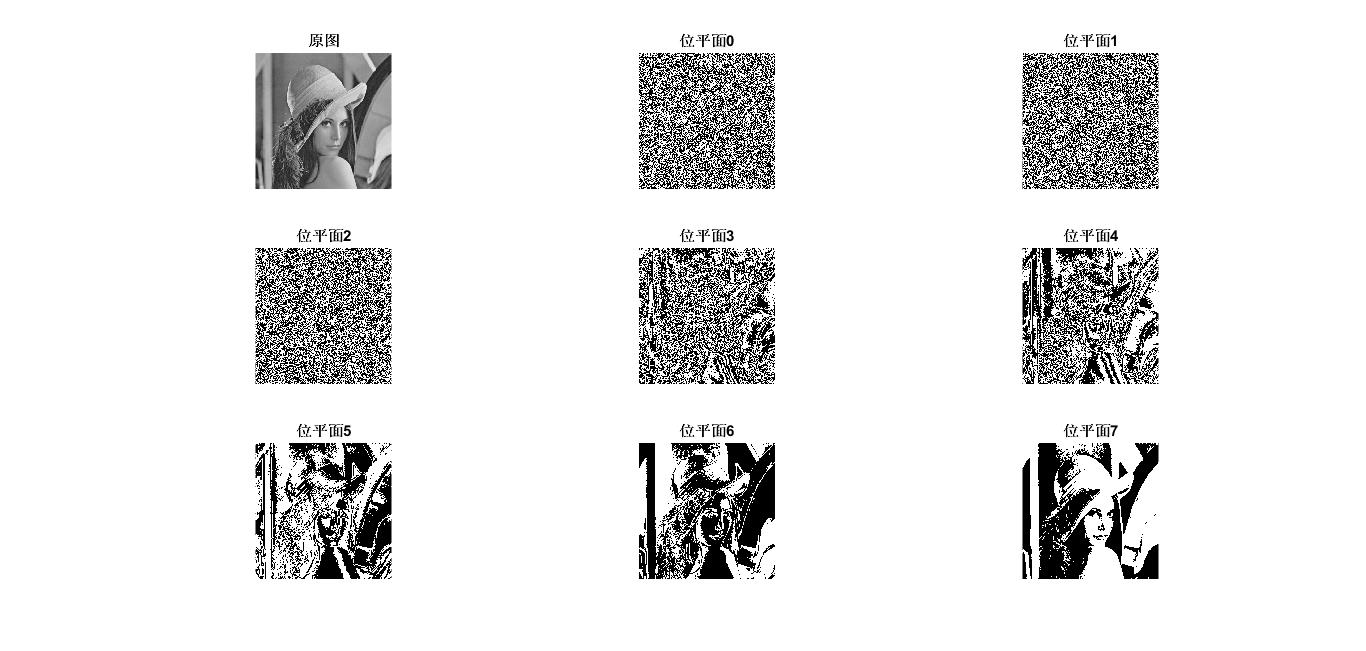
\includegraphics[scale = 0.5]{图像的位分解}
\end{figure}

\subsection{混叠和亚取样}
\subsubsection{混叠效应}
频谱的混叠(Aliasing):取样频率小于奈奎斯特取样频率,或图像为非限带信号,取样图像频率的各次谐波就会发生重叠。

混叠失真:对于已发生混叠的频谱,在图像的恢复中都将会引入一定的失真。

















































































































































































































































































































































































































































































































































































































































































































































































\end{document}